\documentclass[aip, jcp, reprint, onecolumn]{revtex4-2}

\bibliographystyle{apsrev4-2}

\usepackage{physics}
\usepackage{amsmath}
\usepackage{amssymb}
\usepackage{mathtools}
\usepackage{graphicx}
\usepackage{dcolumn}
\usepackage[colorlinks=true, linkcolor=black, urlcolor=blue, citecolor=black, anchorcolor=black]{hyperref}

\graphicspath{{"figures/"}}
\begin{document}
%Title of paper
\title{Coherent IR-Hyper-Raman Four Wave Mixing Vibrational Spectroscopy}


\author{Ryan P. McDonnell} 
\author{Daniel D. Kohler}
\author{John C. Wright} \email{wright@chem.wisc.edu}

\affiliation{Department of Chemistry, 
        University of Wisconsin - Madison, 
        Madison, Wisconsin 53706, 
        United States of America}

\date{\today}

\begin{abstract}
Nonlinear, four wave mixing vibrational spectroscopies are often used to probe intramolecular vibrational coupling and relaxation dynamics in isotropic media.
% Three wave mixing vibrational spectroscopies, such as vibrational sum frequency generation (vSFG) are similarly used to probe the spectroscopy and dynamics of interfacial species.
Most of these methods rely on infrared and/or Raman transitions, but methods involving hyper-Raman transitions are also possible. 
% Implementing a nonlinear spectroscopy involving hyper-Raman transitions can provide a useful analogue to infrared and Raman based nonlinear spectroscopies to understand the spectroscopy and dynamics of isotropic systems.
Hyper Difference Frequency Generation (Hyper-DFG, or HDFG) spectroscopy is an underdeveloped four wave mixing vibrational spectroscopy based on the hyper-Raman transition. 
Despite several experimental reports on HDFG, its spectroscopic properties have not been fully explored.  % DDK: what aspects do we explore?
To this end, we investigate the selection rules and behavior of HDFG spectroscopy.
% We explore the selection rules of singly and doubly resonant HDFG spectroscopy through a Placzek and vibronic picture and show HDFG is a hybrid IR-hyper-Raman technique.
% Since all infrared active modes have non-zero hyper-Raman activity, this makes HDFG a type of upconverted infrared spectroscopy.
% Through a simple comparison test, we demonstrate that HDFG output is shown to be similar in magnitude to vibrational sum frequency generation (vSFG) in a transmission geometry.
% Since HDFG can also be implemented as a two beam experiment in a geometry similar to vSFG, HDFG is a feasible third order spectroscopy for vSFG practitioners.
% Through a simple treatment of orientational averaging, HDFG provides a simple method to extract hyper-Raman hyperpolarizabilities ($\beta$) of infrared active vibrations.
HDFG shows promise as a method to disentangle vibrational spectra and dynamics in isotropic systems.

\end{abstract}

\maketitle

\section{Introduction}
Coherent multidimensional spectroscopy (CMDS) is a family of nonlinear spectroscopy methods that form the optical analogue of multidimensional nuclear magnetic resonance (NMR) spectroscopy.\cite{Cho2008}
Multiresonant, four wave mixing CMDS experiments, first proposed by Oudar and Shen in 1980,\cite{RN307} directly probe coupling and correlations between different vibrational, electronic, and vibronic states. \cite{RN281, RN103, Cho2008} 
Four wave mixing CMDS has resolved anharmonicities, ultrafast dynamics, and other inter- and intra-molecular couplings in numerous systems. \cite{Cho2008, Gaynor2017, Ziegler2018, Ogilvie2019, Bonn2021, RN325}
% DDK: quickly get to vibrational spectroscopy and vibrational-electronic coupling
To target vibrational and electronic coupling, methods commonly make use of Raman transitions (DOVE, TSF, CARS, SRS, RISRS, and citations).
Here we explore the less-utilized hyper-Raman transitions in CMDS four wave mixing spectroscopy.

The hyper-Raman transition is the nonlinear, two photon analogue to the Raman transition.\cite{Terhune1965, Cyvin1965, Andrews1978}
Two photons of frequency $\omega_a+\omega_b$ inelastically scatter with matter, promoting or demoting a vibrational mode of frequency $\omega_v$ and emitting a single photon of frequency $\omega_a + \omega_b \mp \omega_v$.
The single photon emission is a significantly different frequency from the excitation frequencies, making rejection of excitation scatter much easier.
Unlike Raman, all infrared active modes are hyper-Raman active, which allows infrared active modes to be probed through an inelastic scattering event. \cite{Andrews1978}
One drawback is that hyper-Raman transitions are typically weak compared to their Raman counterparts, even when accounting for the high intensities available to ultrafast pulsed lasers.\cite{RN515, Kelley2010}
CMDS methods partially mitigate this issue because emission is spatially coherent so that all emission is directional and easily collected.
In fact, hyper-Raman transitions have been utilized in several CMDS studies.\cite{Zilian1994, RN350, RN416, RN351, RN352, RN353, Chen1998, RN362, RN418, Bonn2024, McDonnell2024,Wang2021}

Hyper-Raman difference frequency generation (HDFG) spectroscopy and hyper-Raman sum frequency generation (HSFG) spectroscopy are four wave mixing CMDS methods based on direct excitation of a vibrational mode through IR absorption and subsequent scattering to or from the vibrational mode through a hyper-Raman transition.
In HDFG/HSFG, an infrared pulse is resonant with a vibrational mode, while two other excitations stimulate the hyper-Raman scattering process.
The infrared excitation frequency selects the vibrational modes to be stimulated through the hyper-Raman transition.
The other two excitation frequencies control electronic enhancement for the scattering event.

\autoref{fig:comparisonwmel} shows both HDFG and HSFG processes and compares it with related spectroscopies that investigate vibrational-electronic coupling.
The three-wave mixing ($\chi^{(2)}$) techniques are often less applicable as they require non-centrosymmetry.
Hyper-Raman scattering itself is a six-wave mixing ($\chi^{(5)}$) technique; stimulated hyper-Raman will be weak and susceptible to FWM cascades (CITE).
Of the many four-wave mixing techniques, HDFG and HSFG have strong similarity to Raman, stimulated Raman, and RISRS in that the electronic state must remove or add a $v$ quantum to the ground state (``ev'' coupling).
With the other four-wave mixing techniques (\autoref{fig:comparisonwmel}, second row), the output signal depends on more states than just the vibrational mode and the electronic state (``evx'' coupling). 
As a result, the relationship between the output and vibrational-electronic coupling is more detailed, but also more complicated.
HDFG, HSFG and Raman are more direct probes of electronic-vibrational coupling.
Notably, HDFG and HSFG can be implemented as 2-color experiments (with $\omega_2=\omega_3$); vSFG or vDFG setups can be trivially reconfigured to perform HSFG or HDFG measurements, respectively, to investigate ev coupling in bulk systems.

When the hyper-Raman excitation is resonant or near-resonant with electronic states, the brightness of the vibrational feature depends on the nature of the electronic state.
The electronic spectrum can inform on processes that control ultrafast electronic relaxation in molecular and biological systems in similar ways to resonance Raman.\cite{Bredenbeck2015, Arsenault2021}
Since the selection rules of hyper-Raman scattering differ from Raman scattering, the hyper-Raman excitation spectra give a unique alternative to Raman scattering to understand vibrational spectra, electronic structure and vibronic coupling in molecular systems. \cite{Olson2018}

% DDK: Quick placeholder caption.  Needs to be refined.
\begin{figure*}[!htbp]
	\centering
	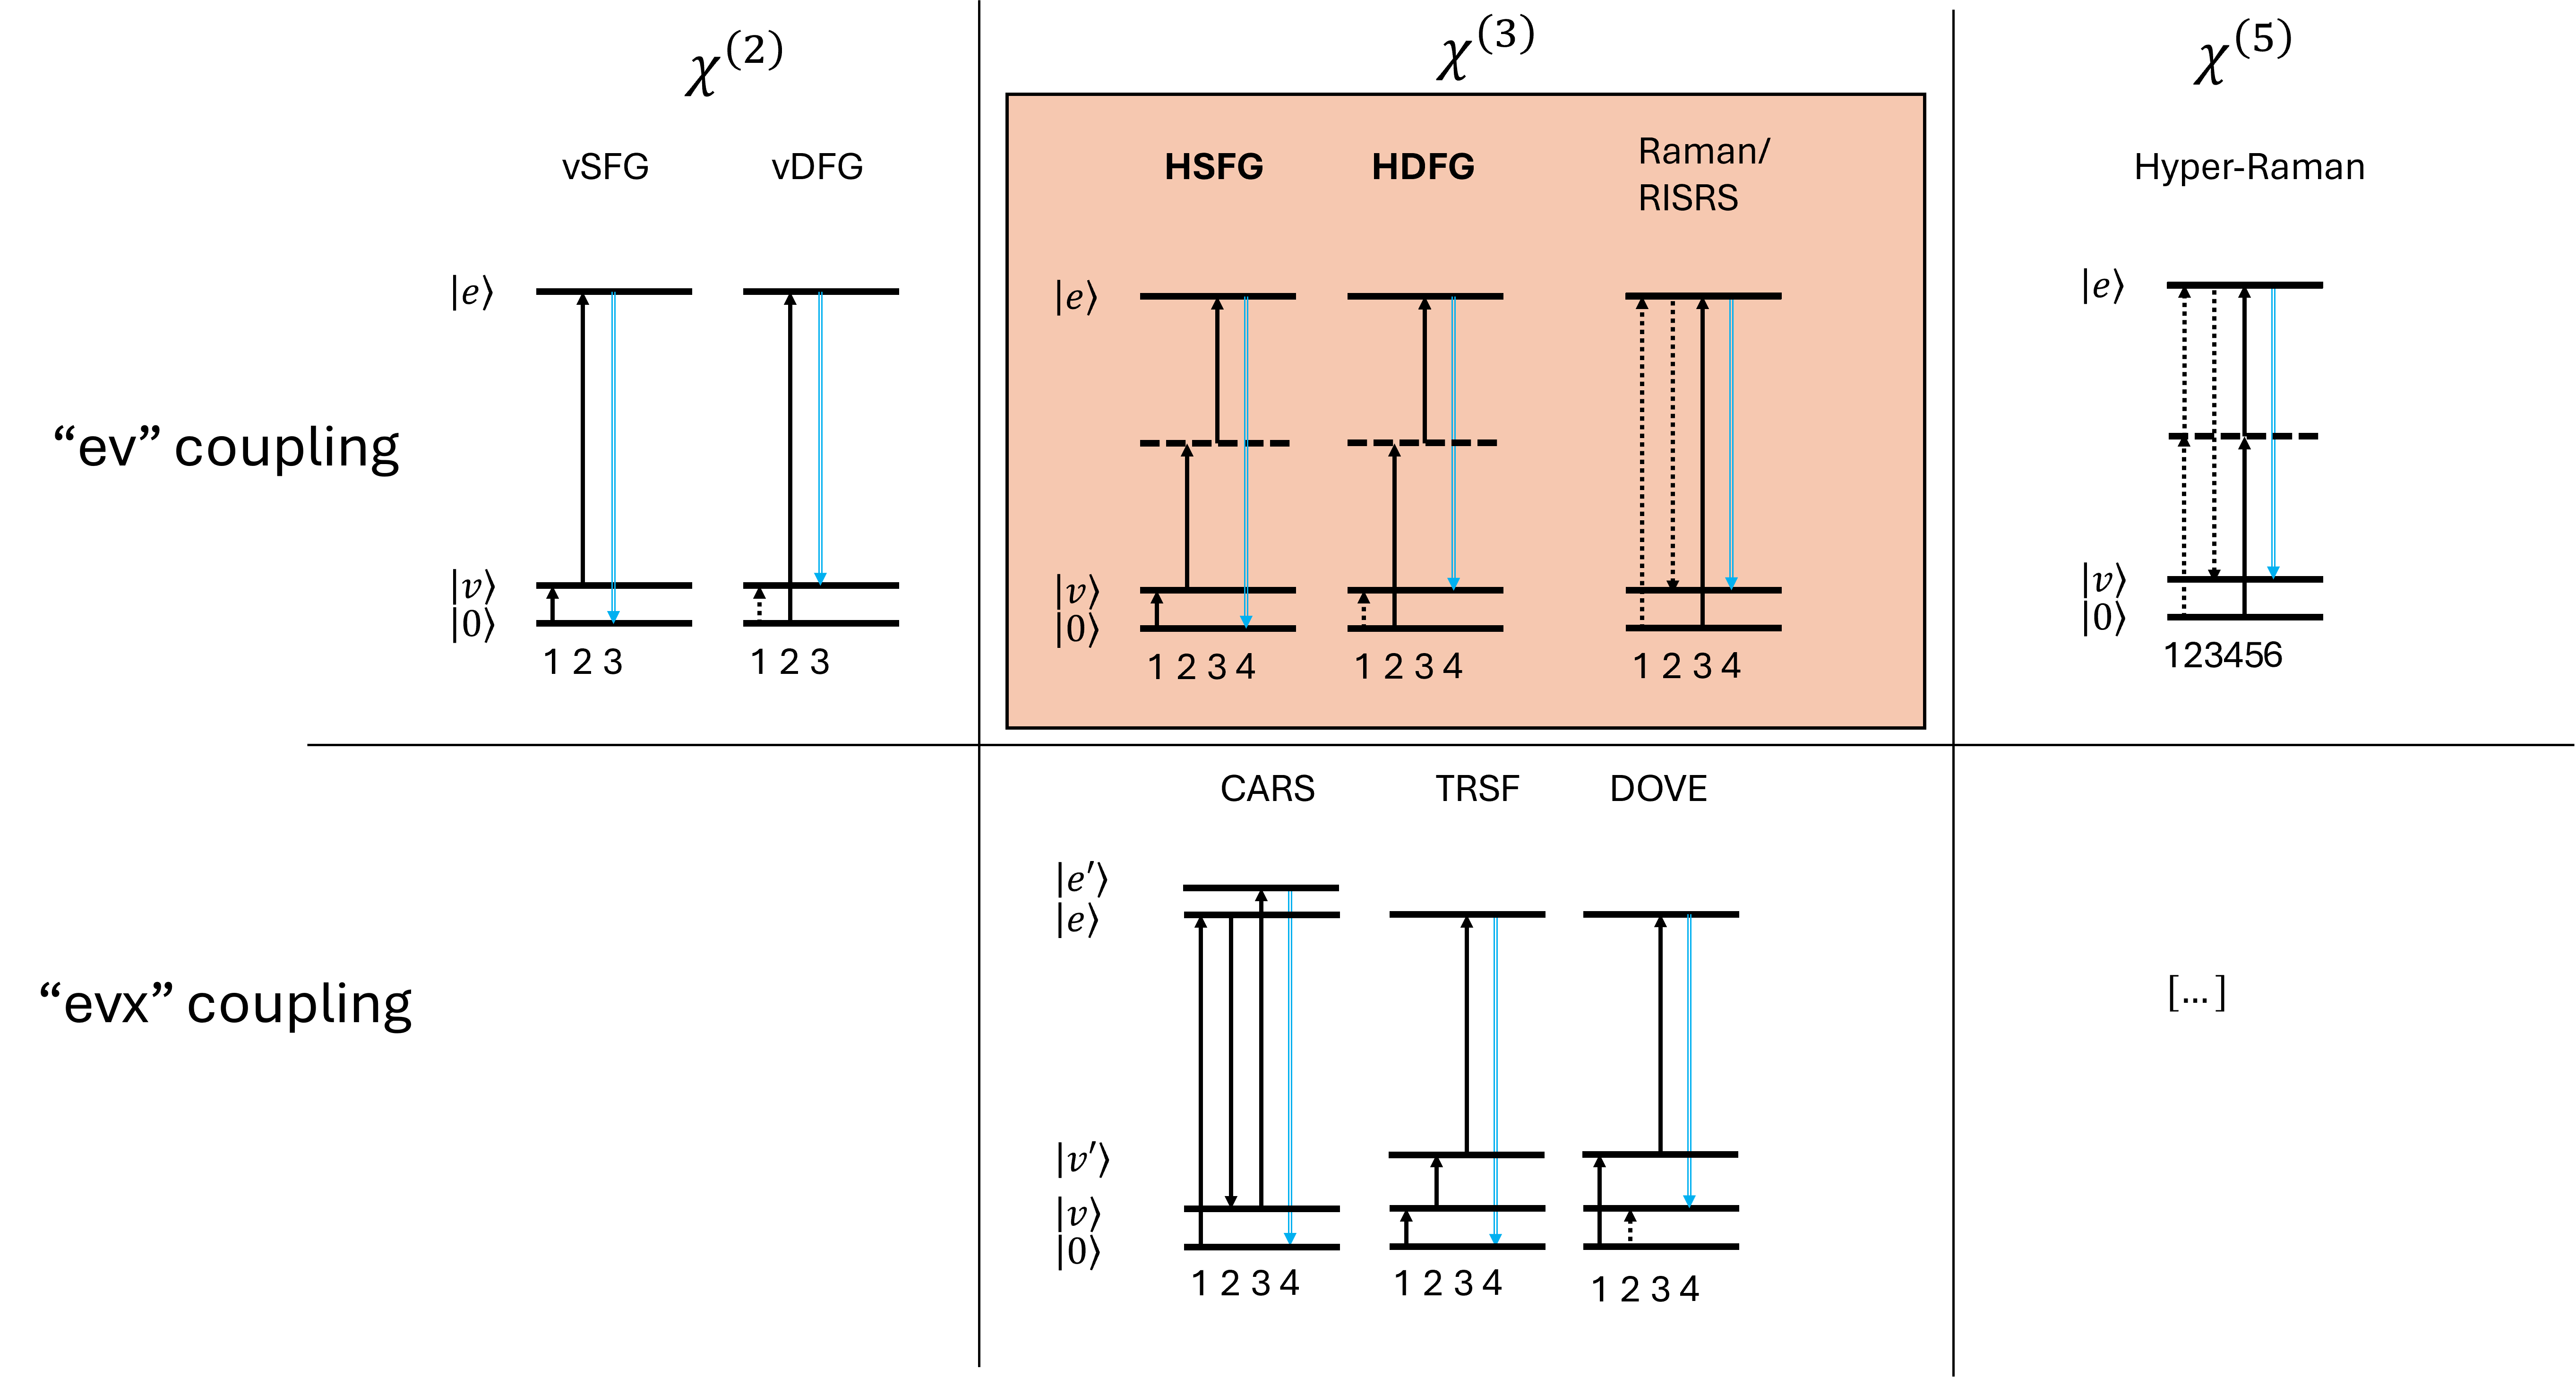
\includegraphics[width=6.66in]{taxonomy.png}
	\caption{
		Spectroscopic methods for investigating vibrational-electronic coupling.
		The interactions of light with matter are shown with Wave Mixing Energy Level (WMEL) diagrams.\cite{RN286}
		Solid and dashed horizontal lines indicate real and virtual states, whereas solid and dotted arrows indicate ket and bra side transitions, respectively. 
	}
	\label{fig:comparisonwmel}
\end{figure*}

Inspired by recent work that demonstrated the presence of HDFG in ultrafast DOVE and terahertz-IR-visible (TIRV) experiments, we investigate the parameters which result in HDFG output. \cite{Cho2000, Bonn2024, McDonnell2024}
This paper is organized as follows.
In \autoref{steadystate}, we first identify the selection rules that drives HDFG in the absence of electronic resonance. 
The selection rules of electronically-resonant HDFG are then identified through the Herzberg-Teller dipole expansion.
Not surprisingly, we find the selection rules are nearly identical to those of hyper-Raman scattering.
A simple harmonic oscillator model system is used to simulate HDFG spectra and illustrate how the excited state potential energy surface affects the hyper-Raman excitation spectrum.
After developing selection rules, the site selective properties and useful experimental aspects of HDFG are discussed in \autoref{quant}.
A new method for extracting hyper-Raman hyperpolarizabilities ($\beta_{ijk}$) from HDFG spectra is identified and discussed.

\section{Selection Rules for HDFG Spectroscopy}\label{steadystate}

% DDK: compiling caveats/scope narrowing statements throughout the paper; to be refined
% Singly resonant hyper difference generation spectroscopy (HDFG) spectroscopy has potential to provide deeper insight into single quantum decoherence times and molecular orientation in condensed systems.
% Similarities between HDFG spectroscopy, infrared spectroscopy and spontaneous hyper-Raman scattering have been noted previously. \cite{RN352, Bonn2024, McDonnell2024}
In this section, we investigate the properties of HDFG and make the connections between HDFG and hyper-Raman scattering explicit.
HSFG will not be discussed, but the application of our treatment to HSFG is straightforward and the information content is similar.
We note that HDFG emission can be phase-matched in media with normal dispersion,\cite{RN278} while HSFG cannot. 

Before presenting selection rules, we note that a potential interferant in HDFG spectroscopy is a sequential cascade of second order DFG and SFG processes.\cite{RN301}
While unimportant in achiral isotropic systems,\cite{Belkin2000} second order cascades may become important in media where SFG and DFG are allowed, e.g. chiral media, interfaces or noncentrosymmetric media. 
Nevertheless, in the discussion that follows for the rest of this manuscript, we will assume negligible second order cascades. % , and use the pathways drawn in \autoref{fig:hdfg} to examine HDFG response. 

It is useful to expose relationships between transition dipoles and hyper-Raman hyperpolarizabilities in the driven limit. \cite{Simpson2004}
Under the electric dipole approximation, the I$^{th}$ component of the third order nonlinear output polarization, ${P}^{(3)}_I$, of a four wave mixing process, induced by electric fields $E_J$, $E_K$, and $E_L$ at output frequency $\omega_4=-\omega_1 + \omega_2 + \omega_3$ is written as (using Einstein summation): \cite{RN307}
\begin{equation} \label{polarization}
{P}^{(3)}_I (\omega_4)  = \chi^{(3)}_{IJKL} E_J(\omega_3) E_K(\omega_2) E_L(\omega_1) 
\end{equation}
where $\chi^{(3)}_{IJKL}$ is the IJKL element of the third order electrical susceptibility, a rank four tensor, generally written as
\begin{equation}
	\chi^{(3)}_{IJKL} = NF(\omega_4) \langle \gamma_{ijkl} \rangle
\end{equation}
where $N$ is a number density, $F$ is the Lorentz local field factor, and $\gamma_{ijkl}$ is the third order polarizability (i.e., second hyperpolarizability). 
The brackets indicate an orientational (or rotational) average.\cite{Andrews1977}
Uppercase letters refer to laboratory frame coordinates and lower case letters refer to corresponding molecular frame coordinates.

% To make the connection between HDFG and hyper-Raman scattering, we investigate its gross selection rules.
% DDK: note that with the current placeholder figure, the state indices will have to be changed in our expressions for e.g. mu, Delta
By propagating density matrix elements in the steady state limit under the rotating wave approximation, the HDFG hyperpolarizability is \cite{RN133}
\begin{equation}\label{sivegamma}
		\gamma_{ijkl}^{vg} =	- \sum_{m, n} \frac{1}{\varepsilon_0} \frac{1}{4D} \frac{1}{\hbar^3} \frac{\mu^{vn}_{i} \mu^{nm}_{j} \mu^{mg}_{k} \mu^{gv}_{l} }{\Delta_{nv} \Delta_{mv}\Delta_{gv}}  \rho_{gg}
\end{equation}
where: $\mu^{ab}_{j}$ is the $j^{th}$ element of $\mel{a}{\vec{\mu}}{b}$, $\Delta_{kl} = \omega_{kl} - \omega_{j} - i\Gamma_{kl}$, $\omega_j$ is the frequency of the j$^{th}$ input field, $\Gamma_{kl}$ is the dephasing of $\rho_{kl}$ and $\rho_{gg}$ is the ground state population.
$D$, the Maker-Terhune degeneracy factor, accounts for permutation symmetry of the excitation fields.\cite{RN134} 
For a HDFG experiment using two (three) distinct input fields, $D = 3 (6)$.

% DDK: or should this be "Vibrational Selection Rules"?  Does Placzek == nonresonant?
\subsection{Electronically Non-resonant: Vibrational Selection Rules}
When $\omega_2+\omega_3$ is significantly detuned from resonance,\cite{Placzek1934, Long1970, Altmann1982} \autoref{sivegamma} 
% DDK: broken thought here
When there is no electronic resonance, HDFG has also been referred to as singly vibrationally enhanced (SIVE) spectroscopy. \cite{RN352}
We first investigate the HDFG selection rules through a Placzek type formalism.
Contracting over the virtual states forms the hyper-Raman hyperpolarizability $\beta$:\cite{Long1970} 
\begin{equation}\label{sivebeta}
	\gamma_{ijkl}^{vg} =	-\frac{1}{\varepsilon_0} \frac{1}{4D \hbar}\frac{\beta^{vg}_{ijk} \mu^{gv}_{l}}{\Delta_{gv}} \rho_{gg}.
\end{equation}
All infrared active transitions are hyper-Raman active, making HDFG allowed for any infrared active transition. \cite{Andrews1978}
This selection rule is generally valid for any HDFG when $\omega_2$ and $\omega_3$ are sufficiently detuned from any resonance.
% It is important to note that the symmetry properties of $\beta_{ijk}$ change dependent upon whether $\omega_2$ and $\omega_3$ are degenerate. \cite{Denisov1986, Kozich2007}  
% DDK: not important, I think?  does this have any bearing on our analysis?

The formula gets simpler when we consider IR excitation of a normal mode.  
Assume state $v$ is the $n^{\text{th}}$ reduced normal mode.
We Taylor expand the dipole and first hyperpolarizability operators to first order in the reduced normal mode coordinate $Q_n$ about equilibrium:\cite{Long1970, Shen90}
\begin{subequations}
	\begin{equation}
		\mu_l = \mu_{l,0} + \left(\frac{\partial \mu_l}{\partial Q_n}\right)_0 Q_n 
	\end{equation}
	\begin{equation}
		\beta_{ijk} = \beta_{ijk,0} + \left(\frac{\partial \beta_{ijk}}{\partial Q_n}\right)_0 Q_n
	\end{equation}
\end{subequations}
Substituting into \autoref{sivebeta} gives the HDFG hyperpolarizability to $\order{Q_n}$ as \begin{equation}\label{SIVEselection}
	\gamma_{ijkl}^{vg} =	-\frac{1}{\varepsilon_0} \frac{1}{8D m_n \omega_{vg}}  \frac{1}{{\Delta_{gv}}} \ \left(\frac{\partial \beta^{vg}_{ijk}}{\partial Q_n}\right)_0 \left({\frac{\partial \mu^{gv}_{l}}{\partial Q_n}}\right)_0  \rho_{gg}
\end{equation}
% DDK: do we call m_n the reduced mass, or the effective mass?
where we have used $\mel{v}{Q_n}{g} = \sqrt{\frac{\hbar}{2m_n\omega_{ng}}}$, $m_n$ is the reduced mass of the normal mode, and $\omega_{ng}$ is the characteristic frequency.\cite{RN230}
Since this expression is non-zero in the harmonic oscillator limit, HDFG output is allowed for normal modes in the harmonic limit. 

% DDK: wait, this is a little different; we are considering w2 as resonant with a vibrational state; we have not considered that yet...
% leaving this out for now
% When electronically non-resonant, there are additional restrictions on the order of the excitation pulses.
% Specifically, when pulse 2 or 3 interacts before pulse 1, and pulse 2 is resonant with a vibrational state, there is interference between competing pathways that is highly destructive.  
% \autoref{fig:hdfg} illustrates the competing pathways; (a) and (b) ((c) and (d)) have the same pulse ordering, but in one pathway pulse 1 stimulates a ket-side transition and in the other a bra-side transition, which imparts a $\pi$ phase shift difference.(CITE) 

\subsection{Electronically resonant and pre-resonant: Vibronic Selection Rules}
% TODO: note that the IR dipole selection rule persists here--this is all about w2+w3 resonance

While the Placzek treatment provides the general source of HDFG output, it does not predict the behavior of $\beta_{ijk}$ as $\omega_2 + \omega_3$ is changed.
We now explicitly consider electronic resonances through the $A,B,C$ decomposition of $\beta$ introduced by Chung and Ziegler, analogous to those found in Albrecht's treatment of Raman spectroscopy.\cite{Albrecht1961, Ziegler1988} 
To employ this formalism, we write the states in a Born-Oppenheimer basis $\ket{a,b}$, where $\ket{a,b} = |a(Q)) \otimes \ket{b}$ for electronic states $\{|a(Q))\}$ and vibrational states $\{\ket{b}\}$ (i.e., adiabatic approximation). \cite{BornOppenheimer, Tang1970}
We will henceforth suppress the dependence of the electronic states on $Q$ for simplicity.
% DDK: can label with fig:comparisonwmel if desired
% The states are labeled as shown in \autoref{fig:hdfg}.
For consistency with previous reports, we use $\vec{R}$ to denote electric transition dipole moments; $\vec{\mu}$ is reserved for transitions on the ground electronic state. \cite{Tang1970}
Following the approach which gave \autoref{sivegamma}, we find
\begin{equation}\label{drgamma_notaylor}
	\gamma_{ijkl} = -\frac{1}{\varepsilon_0} \frac{1}{4D \hbar^3} \sum_{m,n,e,v'} \frac{
		R_{i}^{gv, ev'} 
		R_{j}^{ev',mn} 
		R_{k}^{mn,g0} 
		R_{l}^{g0,gv} 
	}{\Delta_{g0,gv}
		\Delta_{ev', mn}
		\Delta_{mn, g0}
	}
\end{equation}
where $R_{i}^{ab,cd}$ is the i$^{th}$ element of $\mel{a,b}{\vec{R}}{c,d}$.
It is common in the hyper-Raman community to write $\Delta_{ev', mn} \Delta_{mn, g0} = \Delta_{ev', g0}$.
Using our definition of vibronic states, we can write, for example,
$R_{i}^{gv,ev'} = \mel{v}{M_i^{ge}}{v'}$.
Expanding $\vec{M}^{ij}$ to $\order{Q}$ about the equilibrium point of the ground state potential surface as
$\vec{M}^{ij} = \vec{M}^{ij}_0 + \sum_z \frac{\partial\vec{M}^{ij}}{\partial Q_z} Q_z$
yields $A, B, C$ coefficients similar to those in the Albrecht formalism of Raman scattering, \cite{Albrecht1961, Ziegler1988} so that
\begin{equation}
		\gamma_{ijkl} \sim \left(A_{ijk} + B_{ijk} + C_{ijk}\right) \frac{\mel{v}{\mu_{l}}{0}} {\Delta_{g0,gv}}
\end{equation}
The $A$ term contains the static transitions (i.e., Condon approximation), the $B$ term depends upon $\order{Q}$ transitions (Herzberg-Teller contributions), and the $C$ term depends on $\order{Q^2}$ transitions. 
The C term is suppressed in the following discussion as it depends on one and two photon forbidden transitions, making its contribution to $\gamma_{ijkl}$ two orders of magnitude lesser than $A_{ijk}$. \cite{Ziegler1988, Neddersen1989, Bonang1992}
Note that some reports obtain $A, B$ coefficients through a Herzberg-Teller expansion of the electronic states to expose vibronic couplings via $\partial H / \partial Q$, where H is the electronic Hamiltonian.\cite{HerzbergTeller1933, Petrov1985, Neddersen1989, Baranov1990}
This approach is not used here as the expansion of $\vec{M}^{ij}$ in normal mode coordinates provides sufficient physical insight into hyper-Raman selection rules. 

% By contracting over the virtual vibrational states $\ket{n}$, 
The $A$ and $B$ coefficients, where $B = B_1 + B_2$, are written as:
\begin{widetext}
\begin{subequations}\label{ABterms}
\begin{equation}
	\begin{split}
		A_{ijk} = \frac{1}{\hbar^2}\sum_{m,e,v'} M^{ge}_{0,i} 
		M^{em}_{0,j} 
		M^{mg}_{0,k}
		 \langle v | v' \rangle
		 \langle v' | 0 \rangle 
		 \frac{1}{\Delta_{ev', g0}}
		 \\
	\end{split}
\end{equation}
	\begin{equation}
		\begin{split}
			B_{1_{ijk}} &= \frac{1}{\hbar^2} \sum_{m,e,v',z} M^{ge}_{0,i} \langle v | v' \rangle \left(
			 \frac{\partial M^{em}_{j}}{\partial Q_z} M^{mg}_{0,k} \mel{v'}{Q_z}{0} 
			+M^{em}_{0,j} \frac{\partial M^{mg}_{k}}{\partial Q_z} \mel{v'}{Q_z}{0} \right) \frac{1}{\Delta_{ev', g0}}\\
		\end{split}
	\end{equation}
	\begin{equation}
	\begin{split}
			B_{2_{ijk}} = \frac{1}{\hbar^2} \sum_{m,e,v',z} \frac{\partial M^{ge}_{i}}{\partial Q_z} M^{em}_{0,j} 
			M^{mg}_{0,k} \mel{v}{Q_z}{v'} 
			\langle v' | 0 \rangle 
			\frac{1}{\Delta_{ev', g0}}
	\end{split}
	\end{equation}
\end{subequations}
\end{widetext}
where terms such as $\langle a | b \rangle$ and $\mel{a}{Q}{b}$ are Franck-Condon factors and Herzberg-Teller-type integrals, respectively. 
At this point, the expressions are valid for both electronically resonant and non-resonant cases.

For the case of electronic resonance, further simplifications can be made.
We restrict consideration to electronic transitions between $|g)$ and $|e)$.  
% The selection rules for HDFG can be made clearer by small manipulations of \autoref{ABterms}. 
%HDFG (where a vibrational and vibronic state are resonantly coupled) can provide a tool for measuring vibronic coupling, analogous to fully resonant DFG. \cite{Dick83_1, Shen94}
% Many multi-resonant nonlinear spectroscopies have been developed to resolve vibronic coupling in molecular samples. \cite{Carlson1990, Gaynor2017, RN276}
% HDFG provides methods to investigate vibronic coupling with only two laser pulses.
% HDFG experiment selectively excites quanta in ground state vibrational modes, making it similar to a stimulated hyper-Raman experiment. 
% As a result, the spectrum along the electronic scanning axis ($\omega_2 + \omega_3$) is significantly simplified as the coupling between the vibronic states are isolated to only $\ket{g,0}$ and $\ket{g,1}$, assuming the infrared pulse puts a single quantum in the normal mode of interest ($\ket{g,1}$).
By working only in terms of a single normal mode (i.e. removing the sum over $z$ and $v=1$), 
% $v' = \{0,1,2\}$, 
the A and B terms are rewritten as 
	\begin{subequations}\label{ABterms_DR}
		\begin{equation}
			\begin{split}
				A_{ijk} = \frac{1}{\hbar}\sum_{v'} M^{ge}_{0,i} 
				\Lambda^{eg}_{0,jk}
				\langle 1 | v' \rangle
				\langle v' | 0 \rangle 
				\frac{1}{\Delta_{ev',g0}}
				\\
			\end{split}
		\end{equation}
		\begin{equation}
			\begin{split}
				B_{1_{ijk}} &= \frac{1}{\hbar} \sum_{v'} M^{ge}_{0,i} \langle 1 | v' \rangle 
				\frac{\partial \Lambda^{eg}_{jk}}{\partial Q} \mel{v'}{Q}{0} 
				\frac{1}{\Delta_{ev', g0}}\\
			\end{split}
		\end{equation}
		\begin{equation}
			\begin{split}
				B_{2_{ijk}} = \frac{1}{\hbar} \sum_{v'} \frac{\partial M^{ge}_{i}}{\partial Q} 
				\Lambda^{eg}_{0,jk} 
				\mel{1}{Q}{v'} 
				\langle v' | 0 \rangle 
				\frac{1}{\Delta_{ev',g0}}
			\end{split}
		\end{equation}
	\end{subequations}
% DDK: give Lambda an explicit definition, rather than describing it?
where $\Lambda^{eg}_{0,jk}$ is the electronic two photon transition moment between $g$ and $e$.\cite{McClain1977}
$\Lambda$ contains the summation over $m$ in \autoref{ABterms}.

\autoref{ABterms_DR} shows important selection rules for the vibronic transitions.
The $A$ term is allowed whenever an electronic transition has a one- and two- photon transition moment.
The brightness is controlled by vibrational overlap (Franck-Condon factors).
For centrosymmetric molecules, however, an electronic transition cannot be both one- and two- photon allowed, so the $A$ term will vanish.\cite{Milojevich2013, RN230}
This makes HDFG a unique tool for studying the electronic structure of centrosymmetric species in isotropic media, as it is sensitive to non-Condon effects.\cite{Olson2018}
In the absence of an $A$ term, the $B$ terms will dominate.
The $B_1$ and $B_2$ terms involve different types of vibronic coupling pathways.
In $B_1$, the Herzberg-Teller coupling is associated with the two-photon absorption process, whereas in $B_2$, the Herzberg-Teller coupling is associated with one-photon emission.
As such, $B_1$ contributions to a HDFG spectrum will be sensitive to vibronic coupling between the ground state of a mode and vibrational states on the $|e)$ surface. 
$B_2$ contributions are sensitive to vibronic coupling between the first excited state of a mode $\ket{g,1}$ and vibrational states on $|e)$.

\begin{figure*}[!htbp]
	\centering
	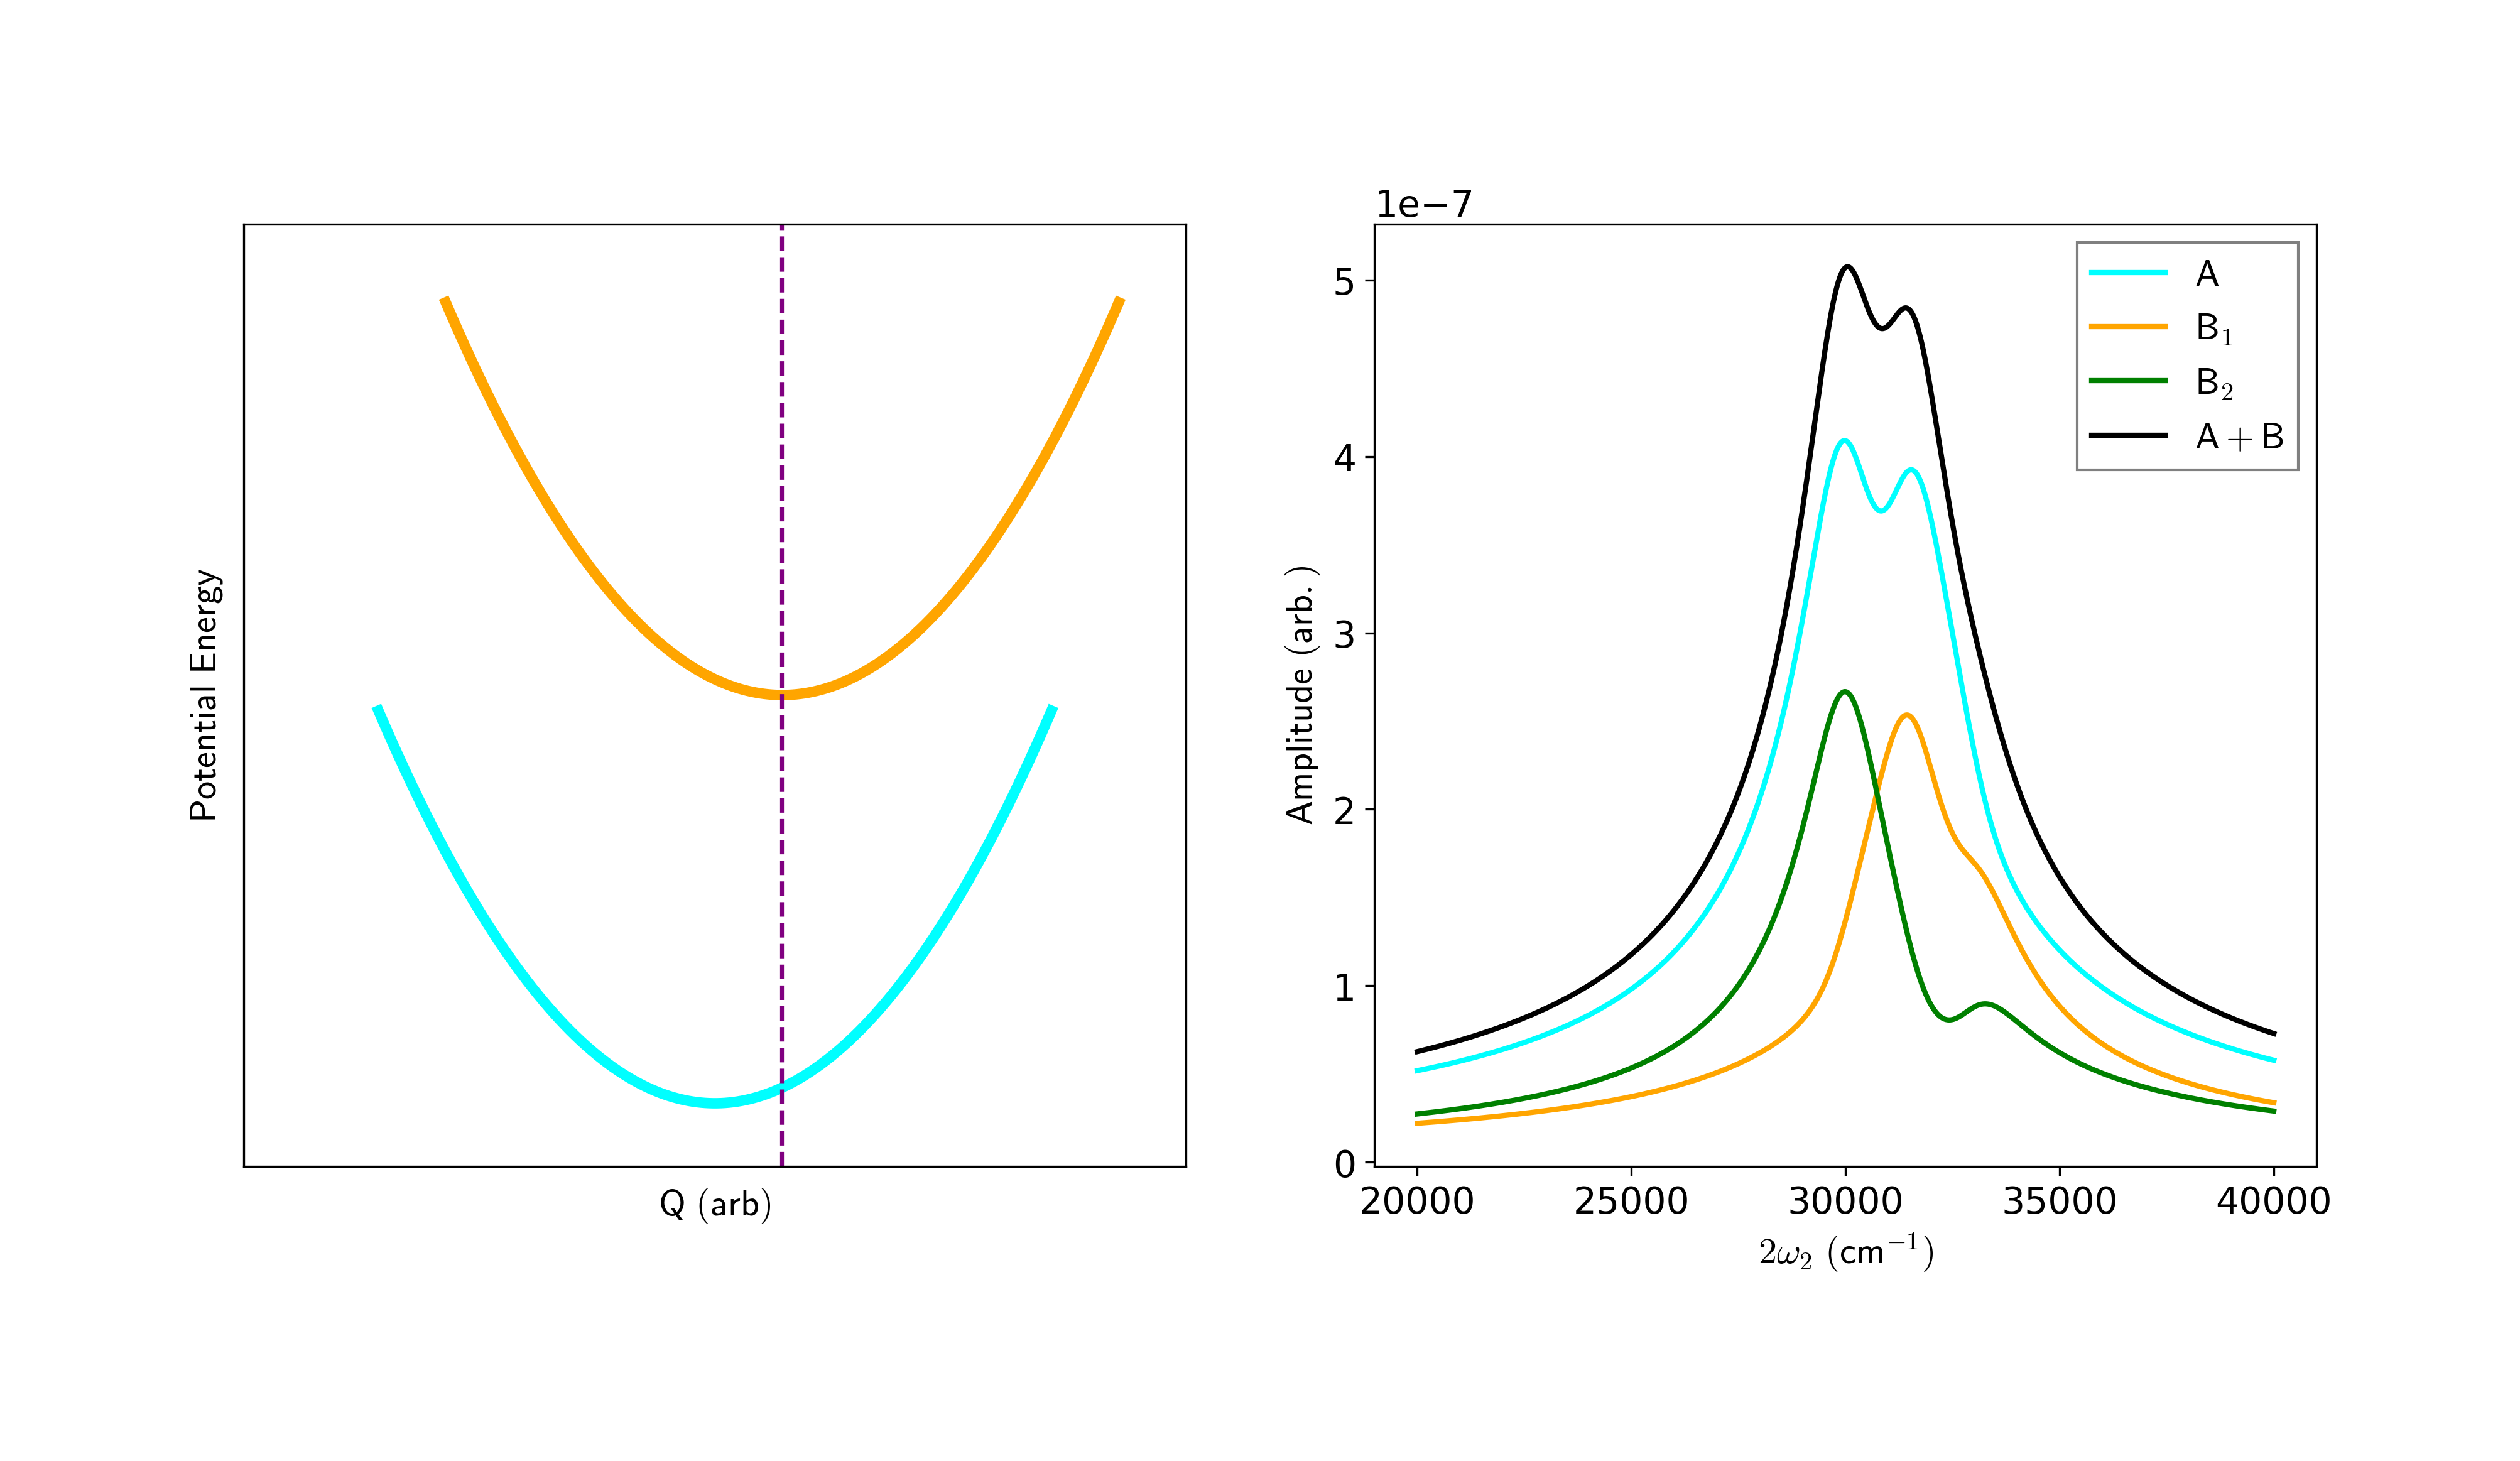
\includegraphics[width=6.66in]{drsive_spectrum.png}
	\caption{Contributions of $A, B$ (\autoref{ABterms_DR}) to HDFG spectrum for a simple two harmonic well system.
		(a) Potential energy surfaces for a two-well system, (b) 1D HDFG spectrum for $\xi = 0.5$, $\omega_1 = \omega_{g1, g0}$. 
		It is assumed that $\omega_2 = \omega_3$.
		Note that (b) plots magnitudes of the labeled quantities.
		The vibrational states on the $|g)$ and $|e)$ manifolds are spaced 2200 cm$^{-1}$ apart, with the vibronic states $\ket{e,v'}$ given linewidths of 700 cm$^{-1}$ and $\hbar \omega_{eg}$ = 30000 cm$^{-1}$.
		Dotted lines in (b) denote the $v'$ = 0, 1, 2 vibronic resonances. 
		The vibronic one and two photon absorption operators are scaled such that $\abs{B}/\abs{A} \sim$ 0.1, following Chung and Ziegler. \cite{Ziegler1988}}
	\label{fig:doubres_spec}
\end{figure*}

The impact of vibronic coupling in the 2D spectrum is made clear by using a simple model. \cite{Kundu2022}
Using a two-well system described by 
\begin{subequations}
	\begin{equation}
		H_g = \frac{p^2}{2m} + \frac{1}{2} \hbar \omega q^2
	\end{equation}
and
	\begin{equation}
		H_e = \frac{p^2}{2m} + \frac{1}{2} \hbar \omega (q-\xi)^2 +\hbar \omega_{eg}
	\end{equation}
\end{subequations}
for the ground ($H_g$) and first excited ($H_e$) states, where $p$ is the momentum of the normal mode, the A and B contributions can be evaluated using Franck-Condon and Herzberg-Teller integrals tabulated in terms of the dimensionless normal mode $q$ and offset parameter $\xi$ (\autoref{fig:doubres_spec}a). \cite{Carlson1988thesis} 
Note that $q = \sqrt{\frac{m^2\omega}{\hbar}} Q$.
The spectrum is simulated for an electronic state which is both one and two photon allowed.
A simulated spectrum (\autoref{fig:doubres_spec}b) highlighting the contributions of these terms on potential wells with $\xi = 0.5$ dissects the $A$ and $B$ contributions to the HDFG spectrum.
This stimulated hyper-Raman type spectrum would be the expected result in a HDFG experiment when investigating the vibronic structure of the electronic state coupled to $\ket{g,v}$.

Simulating the HDFG spectrum for the simple two-well system allows dissection of selection rules and spectral signatures without the need for complex couplings.
There are two relevant regions of interest: the resonant region (2$\omega_2$ $\in$ [29000, 35000] cm$^{-1}$) and the non-resonant region.
Focusing far away from the resonant region ($2\omega_2 \sim$ 20000 cm$^{-1}$), the nonresonant $A$ term response is roughly equivalent to that of the resonant $B$ term response. 
Previous reports suggest that $A$ term contributions may become negligible when significantly detuned from a resonance such that $\Delta_{ev', g0} \approx \Delta_{eg}$, i.e., the resonance denominator loses $\ket{v'}$ dependence. \cite{Neddersen1989}
The lack of $\ket{v'}$ dependence in the resonance denominator causes $A$ to vanish through closure ($A_{ijk} \sim \sum_{v'} \langle 1|v' \rangle \langle v'|0\rangle$ = $\delta_{10} = 0$).
However, the simulated spectrum (\autoref{fig:doubres_spec}b) shows a non-negligible $A$ contribution to HDFG output well beyond $\sim$ 20000 cm$^{-1}$, the limit for this model system where $\abs{\omega_{ev',g0} - 2\omega_2} \gg 2\Gamma_{ev',g0}$.
As such, it is difficult to eliminate $A$ term resonances in HDFG spectra, even when largely detuned ($\gg 2\Gamma_{ev',g0}$) from the electronic state. 
Similar ideas have been seen in spontaneous Raman scattering. \cite{Li1990, Gong2015}
As such, it may prove difficult to examine non-Condon effects in HDFG spectra of noncentrosymmetric systems. 

In the resonant region, the $A$ term contains character from all three possible transitions between $\ket{g,0}$, $\ket{e,v'}$ and $\ket{g,1}$. 
Significant contributions from $\ket{e,0}$ and $\ket{e,1}$ in the spectrum correspond well with expectations given the relative wavefunction overlap in \autoref{fig:doubres_spec}a. 
The small contribution to $A$ involving transitions with $\ket{e,2}$ is consistent with the large change in quantum number from $\ket{g,0}$ and its considerable displacement from the equilibrium point of $|g)$.
The dependence of $A$ on these Franck-Condon factors is in agreement with expectations following \autoref{ABterms_DR}. 

Unlike $A$ term contributions, the $B_1$ and $B_2$ terms are dependent upon both Franck-Condon and Herzberg-Teller contributions.
Based upon the disparity in transition amplitudes in the $B_1$ and $B_2$ terms for each vibronic transition, it is clear that the $B$ terms are sensitive to the Herzberg-Teller coupling integrals.
The $B_1$ term, whose vibronic coupling term is involved in the two-photon absorption event from $|g)$ to $|e)$, seemingly has minimal $0-0$ contributions. 
This is expected, as the Herzberg-Teller integral $\mel{0}{Q}{0}$ is smaller than $\mel{1}{Q}{0}$ and $\mel{2}{Q}{0}$. 
An explanation for the contribution from the $0-1$ transition in $B_2$ is similar.
Vibronic contributions to $B_2$ arise from the one photon emission transition; $\mel{1}{Q}{1}$ is smaller than the $\mel{1}{Q}{0}$ and $\mel{1}{Q}{2}$ contributions to the $B_2$ term.
However, the $0-2$ transition is smaller in amplitude than the $0-1$ transition because it is also dependent upon a $\langle 2 | 0 \rangle$ Franck-Condon factor.
In a realistic molecular system, where higher order contributions (e.g. Duschinsky coupling) affect vibronic coupling signatures, the spectral signatures will change to incorporate anharmonicites. \cite{Duschinsky1937, Carlson1990, Kundu2022}
Investigating coupling between $\ket{g,2v}$ and the same $\ket{e,v'}$ vibronic states will likely assist in dissecting the site-selective electronic spectra.

\section{Comparisons with other spectroscopies}\label{quant}
\subsection{Site Selectivity}
Unlike resonant hyper-Raman spectroscopy, which allows transitions between different normal modes of varying quanta, the infrared pulse in the HDFG provides a type of site selectivity,\cite{RN103, Carlson1991} so that only the mode pumped by $\omega_1$ can be involved in vibronic coupling.  
% DDK: I kind of understand this point...but a hyper-Raman spectrum would clearly select the vibrational mode based on the Raman shift, correct?
%  good to note the benefits of this technique compared to hyper-Raman:
% - a form of stimulated hyper-Raman (=stronger, directional signals)
% - experiment takes place over a short time window, so pump-probe experiments are easily implemented
% - laser scatter is easily avoided
% - IR active, not 
HDFG methods can supplement other coherent Raman based methods as a method to investigate vibronic coupling mechanisms between a specific vibration on the ground state and vibrational states on an arbitrary excited state.\cite{RN103}
The combined infrared and hyper-Raman properties of HDFG make it highly sensitive to molecular electronic structure.
Particularly in the case of a centrosymmetric species, non-Condon effects dominate in the spectrum as the $A$ term vanishes from the presence of an inversion center.
The site selective properties of HDFG can allow for parsing of non-Condon effects in different vibrational modes, and extend the use of CMDS to understand the electronic and vibronic structure of simple and complex species.

The hybrid infrared / hyper-Raman properties of HDFG make it an intriguing analogue of resonance IR spectroscopy.
First demonstrated by Boyle et al., resonance IR uses a $2\vec{k}_1 + \vec{k}_3$ pathway to amplify weak infrared modes through vibronic coupling, dependent upon the Raman $A,B$ coefficients. \cite{RN491}
However, the $2\vec{k}_1 + \vec{k}_3$ resonance IR method implicitly depends upon the coupling of an overtone $\ket{g,2v}$ to vibronics $\ket{e,v'}$.
% DDK: did we not already discuss this?  Why is this not the introduction?
Alternatively, HDFG provides another form of resonance IR spectroscopy, but only requires coupling between $\ket{g,v}$ and $\ket{e,v'}$.
This form of resonance IR spectroscopy would also uniquely depend upon one and two-photon absorption components, as discussed in terms of the hyper-Raman $A,B$ coefficients.
By combining resonance IR in the HDFG and $2\vec{k}_1 + \vec{k}_3$ geometries, the sensitivity of the Raman and hyper-Raman $A,B$ coefficients to ground state vibrations and electronic structure can be assessed. 
Such experiments can help assess the quality of computationally calculated ground and excited state potential energy surfaces. 

\subsection{Comparison to Sum Frequency Generation}
% this whole argument is we only need two colors...condense this
% also note the intro covers this now
Despite these attributes of HDFG, four wave mixing techniques are usually unfeasible for most laboratories, as they usually demand the use of multiple optical parametric amplifiers and/or complex acousto-optic modulators. \cite{RN245}  % I don't understand the citation, but also a citation is not necessary...
Unlike most four wave mixing techniques, HDFG can be performed using only two input beams (i.e., two color HDFG).
In the case of two color HDFG, only one tunable infrared optical parametric amplifier is needed, as the oscillator which pumps the infrared OPA can be used to perform the two-photon upconversion needed to generate HDFG output, i.e., $-\vec{k}_1 + 2\vec{k}_2$.
A commonly used two laser CMDS method is vibrational sum frequency generation (vSFG), a $\chi^{(2)}$ technique whose phasematching is dictated by $\vec{k}_1 + \vec{k}_2$.
vSFG output scales as $\chi^{(2)}_{IJK} \sim \langle \alpha_{ij} \mu_k \rangle$, where $\alpha_{ij}$ is the Raman polarizability tensor.
Laboratories which use vSFG to investigate interfacial species at buried interfaces thus have the ingredients necessary to perform a HDFG experiment in a transmission geometry. \cite{Piontek2023_1}
This would allow vSFG practitioners to perform measurements in the bulk, such as measuring free induction decay, vibrational population lifetimes, and steady-state vibrational spectra through HDFG.
 
Assessing the relative amplitudes of vSFG and HDFG is useful for demonstrating its feasibility as a nonlinear infrared spectroscopy. 
Note that both vSFG and HDFG can be phasematched in media with normal indices of refraction, unlike the $\vec{k}_1 + 2\vec{k}_2$ HSFG process (\autoref{fig:comparisonwmel}).\cite{RN120}
Macroscopically, oddness in spatial inversion of the vSFG polarization eliminates output from centrosymmetric species under the electric dipole approximation.\cite{RN132, RN133}
As a result, vSFG output is significantly reduced relative to most third order spectroscopies because it depends on surface number density, many orders of magnitude smaller than the bulk surface density. 
% DDK: we should clarify that these cross sections are weak even for non-linear cross-sections
Hyper-Raman cross-sections are commonly several orders of magnitude weaker than corresponding Raman transitions.\cite{RN515}

% As a result, it is important to compare the relative output polarizations for both vSFG and HDFG taking into account the significant disparities in number densities and oscillator strengths. 

% DDK: put this calculation in the SI; it's not really important.
% To motivate the application of HDFG spectroscopy in a vSFG type geometry, we perform a calculation to compare two-color HDFG and vSFG output, where absorption effects are neglected for simplicity.
% The output polarizations under the electric dipole approximation are written as
% \begin{widetext}
% 	\begin{subequations}
% 	\begin{equation}\label{PSFG}
% 		\abs{P^{(2)}_{\text{vSFG}}} = \frac{N_{surf}}{\ell} F(\omega_1+\omega_2) \abs{\langle \alpha_{ij}\mu_{k} \rangle E(\omega_2)E(\omega_1)} 
% 	\end{equation}
% 	\begin{equation}
% 		\abs{P^{(3)}_{\text{HDFG}}} = N_{bulk}  F(2\omega_2-\omega_1) \abs{\langle \beta_{ijk} \mu_{l} \rangle E{(\omega_2)}E(\omega_2)E(-\omega_1)}
% 	\end{equation}
% \end{subequations}
% \end{widetext}
% where N$_{bulk}$ is the bulk number density ($\sim$ 10$^{28}$ m$^{-3}$ for H$_2$O$_{(l)}$ at room temperature), and N$_{surf}$ is the surface number density ($\sim$ 10$^{16}$ m$^{-2}$ for H$_2$O adsorbed at quartz).\cite{Du1994}	
% For simplicity, we assume that $\chi^{(2)}$ is a spatial constant so that $\int_{0^-}^\ell \mathrm{d}z \langle \alpha_{ij}\mu_{k} \rangle \approx \ell \langle \alpha_{ij}\mu_{k} \rangle$, where $z$ is oriented along the surface normal and $0^{-}$ is the edge of the interface where substrate begins. \cite{Su1998}
% We take the film thickness ($\ell$) probed by vSFG to be 1 nm, much less than the vSFG coherence length.\cite{RN133}
% A normal dispersion curve is assumed so that $F(\omega_1+\omega_2) \approx F(2\omega_2-\omega_1)$.
% To simplify analysis, orientational averaging is ignored (e.g., $\langle \beta_{ijk} \mu_{l} \rangle \approx \beta \mu$) and the input and output fields are taken to be co-polarized, so that
% \begin{equation}
% 		P_{ratio} \equiv \frac{\abs{P^{(3)}_{\text{HDFG}}}}{\abs{P^{(2)}_{\text{vSFG}}}} \approx \frac{N_{bulk}}{N_{surf}} \frac{\beta}{\alpha} E(\omega_2) \ell \sim 10^3 \frac{\beta}{\alpha} E(\omega_2)\\
% \end{equation}
% Ziegler has noted that for a field with intensity 10 GW/cm$^{2}$, $\frac{\beta E}{\alpha} \sim 10^{-3} $ for vibrational modes when $E(\omega_2)$ is largely detuned from electronic resonances. \cite{RN515}
% Such an intensity is easily obtained using modern ultrafast sources.
% In this limit, $P_\text{ratio} \sim 1$.
% Since the intensity ratio scales as $\abs{P_{ratio}}^2$, we see that the HDFG output is roughly as strong as vSFG, assuming only interfacial contributions in vSFG.
% It is important to note that this calculation assumed negligible dipole and Raman polarizability dependence upon the distance from surface normal, ignored orientational averaging effects, and presumed equivalence of local field factors, all of which can significantly reduce output from either process. 
% Nevertheless, since HDFG produces a number of photons similar to that of vSFG, HDFG is a viable technique for investigating bulk systems.
% This method provides practitioners of sum frequency generation the ability to probe isotropic dephasing dynamics without many meaningful changes in their optical setup, and thus compare  dephasing in the bulk and at the interface.\cite{RN224}

Transient HDFG spectroscopy, or pump-HDFG-probe, similar to transient vSFG spectroscopy (pump-vSFG-probe), can be implemented to learn about relaxation dynamics in isotropic systems. \cite{RN224, Bonn2024}
A useful attribute of the $\beta_{ijk}$ dependence in HDFG output is added polarization control. 
Similar to SFG experiments that probe different elements of the infrared transition dipole and Raman polarizability tensors, probing different elements of $\beta_{ijk}$ in HDFG can greatly assist in understanding ultrafast dynamics in isotropic systems, as suggested by Seliya et al. \cite{Shen90, RN224, Bonn2024}
Polarization control in IR-pump-HDFG-probe, analogous to polarization control in pump-vSFG-probe, would be an interesting venue to assess the sensitivity of HDFG to different hyper-Raman tensor elements, and for practioners of transient vSFG to compare polarization specific dynamics at the interface and in the bulk. 

\subsection{Quantitative HDFG: Measuring the Hyper-Raman Hyperpolarizability}
With the selection rules of HDFG understood for vibrational spectroscopy, and with HDFG generating a large enough output polarization, it becomes possible to obtain quantitative information from its spectra.
Lineshape analysis is essential for extracting quantitative information from CMDS spectra.
Scanning across resonances create dispersive lineshapes, i.e, self-heterodyning, which inform on $\Re(\chi^{(3)})$ and $\Im(\chi^{(3)})$.\cite{Levenson1974_1, Levenson1974_2}
In the method introduced by Levenson and Bloembergen (Bloembergen Interferometry Experiment), an internal standard interferes with the resonant lineshape.
Self-heterodyning of the internal standard signal measures $\chi^{(3)}$ and does not require measurement of absolute intensities. 
Resonant lineshapes are also complicated by amplitude level interference between the sample,  substrate and/or sample cell windows, which must be accounted for to obtain quantitatively correct $\chi^{(3)}$ values. \cite{RN362, RN418}
Most quantitative methods in an n$^{th}$ order CMDS experiment are used to measure $\chi^{(n)}$ values to compare the relative strength of nonlinear processes in different media. \cite{Zhu87, RN351, RN345}
The recorded $\chi^{(n)}$ values provide insight into how microscopic quantities ($\vec{\mu}, \alpha_{ij}, \beta_{ijk}$) impact nonlinear output.
These quantities are usually measured using their incoherent analogues (IR spectroscopy, spontaneous Raman spectroscopy, spontaneous hyper-Raman spectroscopy). \cite{Levenson1974_2, RN412, Shoute2005}

Compared to $\vec{\mu}$ and $\alpha_{ij}$, it is difficult to calculate $\beta_{ijk}$ values from spontaneous hyper-Raman experiments. \cite{Kelley2010}
Only a few experimental determinations of $\beta_{ijk}$ for vibrational modes have been performed. \cite{Xu1997, Shoute2005, Kelley2010}
Methods reported in the literature to measure absolute hyper-Raman polarizabilities depend upon external standards such as hyperpolarizabilities of dissolved samples or two-photon absorption cross sections, also difficult to measure.
Since the Bloembergen interferometry experiment only relies on the third order susceptibility for measured species (e.g., benzene or CaF$_2$),\cite{Levenson1974_2} it is possible to use quantitative four wave mixing spectroscopy to calculate $\beta_{ijk}$ values.
It is thus useful to investigate how a treatment of orientational averaging can extract $\beta_{ijk}$ from the HDFG $\chi^{(3)}_{IJKL}$ expression.

In HDFG, 
\begin{equation}\label{chi3}
\begin{split}
		\chi^{(3)}_{IJKL} &= NF(\omega_4) \langle \gamma_{ijkl} \rangle = -\frac{NF}{4D \hbar \varepsilon_0 \Delta_{gv}} \langle \beta_{ijk} \mu_l \rangle \rho_{gg}\\
\end{split}
\end{equation}
For simplicity, we take $\rho_{gg} = 1$.
The steps behind orientational averaging of $\gamma_{ijkl}$, a rank four tensor in the molecular frame, are detailed elsewhere.\cite{Andrews1977, McDonnell2024}
Briefly, a tensor in the molecular frame, A$_{ijkl}$, is transformed into an element of the same tensor in the laboratory frame, A$_{IJKL}$, through A$_{IJKL}$ = $\theta^{ijkl}_{IJKL} A_{ijkl} = \langle A_{ijkl} \rangle$, where summation over repeated indices is implied and $\theta$ is the transformation operator. \cite{McDonnell2024}
Orientational averaging shows specific polarization schemes isolate linear combinations of different $\beta_{ijk}$ terms. \cite{Bersohn1966, Willetts1992, Kauranen1996}
By using the expansions of $\beta_{ijk}$ and $\mu_{l}$ to $\order{Q_n}$ found earlier, and knowing that $\Re(\chi^{(3)})$ vanishes when resonant, we see
\begin{equation}\label{betasive}
	\left\langle \frac{\partial \beta_{ijk}}{\partial Q_n} {\frac{\partial \mu_l}{\partial Q_n}} \right\rangle = -\frac{8D \varepsilon_0}{NF}  {\Gamma_{gv} \omega_{vg}} {\Im(\chi^{(3)}_{IJKL})}
\end{equation}
Since $\abs{\partial \mu / \partial Q}$ values can be extracted from FT-IR spectra, HDFG can give quantitative information on the magnitude of $\beta_{ijk}$ for infrared active vibrations.
Additionally, by using non-degenerate input frequencies to stimulate the hyper-Raman transition, the asymmetric properties of $\beta_{ijk}$ can be examined and quantified. \cite{Christie1971, Denisov1986, Kozich2007}
To our knowledge, no experiment has been performed which quantifies deviations of the asymmetric and symmetric components of $\beta_{ijk}$. 
These quantitative aspects of HDFG could prove useful to examine how well computational methods calculate $\beta_{ijk}$ values and the strength of spontaneous hyper-Raman scattering with non-degenerate pulses.

\section{Conclusions}
Coherent vibrational, hyper-Raman coherent four wave mixing spectroscopies are identified and discussed.
Singly resonant hyper difference frequency generation (SR-HDFG) processes are shown to be the coherent hyper-Raman analogue of infrared active vibrations.
We find that HDFG is always allowed for harmonic transitions, making it a potential tool for measuring single quantum coherence lifetimes. 
Through an examination of the hyper-Raman $A,B,C$ terms, the impact of electronic resonance and vibronic coupling in HDFG spectrum was examined.
The non-Condon effects that are present in the absence of $A$ might prove useful for resolving the electronic structure of centrosymmetric species.
HDFG possesses types of site-selective properties analogous to those of nanosecond coherent Raman experiments. 
Site-selective properties should allow for a thorough analysis of vibronic coupling schemes in isotropic systems.
Through a simple treatment, it is seen that HDFG and vibrational sum frequency generation (vSFG) have roughly the same output intensities. 
This makes HDFG a reasonable spectroscopy for systems outside of the ideal solvents tested in the literature, and should be readily extended to a variety of non-ideal molecular and materials systems. 
Based upon a simple treatment of orientational averaging, we show that HDFG can extract the hyper-Raman hyperpolarizability without a need for technically difficult, analytically rigorous hyper-Raman scattering experiments. 
The HDFG method shows promise as a spectroscopic probe of unique electronic structure effects in a variety of molecular systems, but also for understanding the dynamics of single quantum coherences. 
\section{Data Availability}
The workup scripts which support this work can be found at [insert github link here].

\section{Acknowledgments}
This work received support from the Department of Energy, Office of Basic Energy Sciences, Division of Materials Sciences and Engineering (Grant no. DE-SC0002162).
R.P.M. acknowledges support from the NSF Graduate Research Fellowship Program (Grant no. DGE-2137424). 

%todo: figure out how footnotes work...

%{By defining $\Lambda^{mn}_{ij} = \sum_k (m|M_i|k) (k|M_j|n)$, expanding $\Lambda^{mn}_{ij}$ to $\order{Q}$ gives $\Lambda^{mn}_{0,ij} + \partial/ \partial Q \sum_k (m|M_i|k) (k|M_j|n) Q$ = $\Lambda^{mn}_{0,ij} + \sum_k (m|\partial M_i / \partial Q|k) (k|M_j|n) Q + (m|M_i|k) (k|\partial M_j / \partial Q|n) Q$, in agreement with the substitution made above.} 

\section{References}
% Create the reference section using BibTeX:
\bibliography{library.bib}

\end{document}
%


